
\chapter{Regra do MIT}
\section{Parâmetros}
Escolhemos um modelo de planta de segunda ordem da seguinte forma:
\begin{equation}
G(s) = \frac{b[1]*s + b[0]}{s^2 + a[1]s + a[0]}
\end{equation}

Com $b$ = [11 0] e $a$ = [11 10], de forma que os polos da planta são -1 e -10. O modelo de referência foi escolhido de forma a aumentar o valor em módulo dos polos da planta em 25 porcento e manter o ganho em regime permanente para referência do tipo degrau. De forma que temos o seguinte modelo:

\begin{equation}
G_m(s) = \frac{1.5625b[0]}{s^2 + 1.25a[1]s + 1.5625a[0]}
\end{equation} 

Definimos o erro de saída $e_0$ entre a planta e o modelo de referência, onde $y(t)$ é a saída da planta e $y_m(t)$ a saída do modelo:

\begin{equation}
e_0 = y(t) - y_m(t)
\end{equation}

A partir dos argumentos padrão para controle adaptativo direto, chegamos às leis adaptativas usando a regra do MIT:

\begin{equation}
\dot{\theta}_1 = \gamma_1 e_0 y_f
\end{equation}

\begin{equation}
\dot{\theta}_2 = \gamma_2 e_0 \dot{y}_f
\end{equation}

\begin{equation}
\dot{\theta}_3 = -\gamma_3 e_0 r_f
\end{equation}

Onde o índice $f$ denota a passagem do sinal por um filtro determinado pelo modelo de referência escolhido. Usamos $\gamma_1 = 1$, $\gamma_2=1$ e $\gamma_3=1$, e condições iniciais para a planta e modelo da forma:

\begin{equation}
\theta_m(0) = [0~;~2]
\end{equation}

\begin{equation}
\theta_p(0) = [-4~;~3]
\end{equation}

\section{Resultados}

Observamos na figura 1.1 o erro de saída da planta, para uma referência degrau.\\


 \begin{figure}
 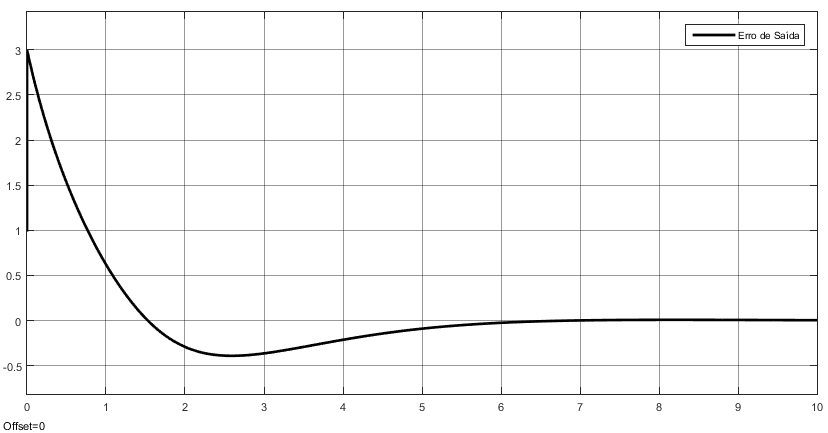
\includegraphics[width = 15 cm, height = 9 cm]{./pics/Erro_de_saida_MRAC_MIT_10seg.png}
 \caption{Erro de Saída da Planta, 10 segundos de simulação}
 \end{figure}

Na figura 1.2, para 10000 segundos de simulação, observamos a convergência das estimativas dos parâmetros da planta no espaço de parâmetros para seus valores corretos, dada uma entrada persistentemente excitante:

\begin{figure}
 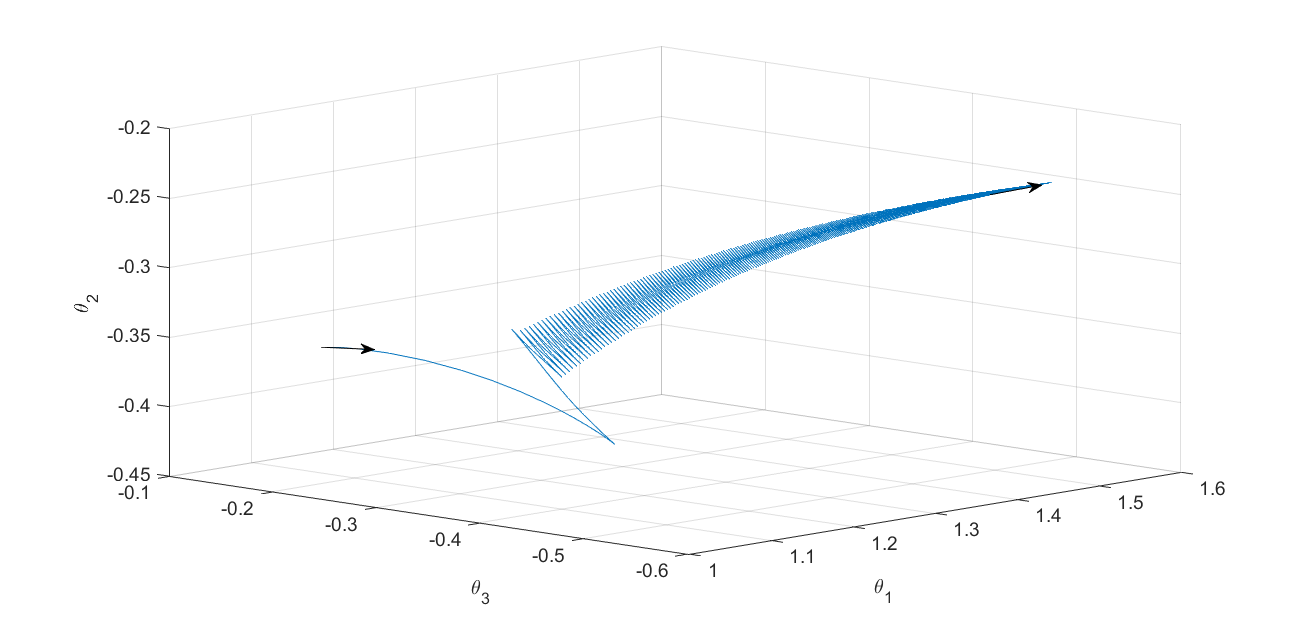
\includegraphics[width = 15 cm, height = 9 cm]{./pics/Trajetoria_MRAC_MIT_10000seg.png}
 \caption{Trajetória das estimativas dos parâmetros da planta, 10000 segundos de simulação}
\end{figure}

\chapter{Método do Gradiente}

Com a mesma planta usada nas simulações anteriores, definimos o erro entre a saída da planta e a estimativa para a saída da planta:

\begin{equation}
\varepsilon = y - \hat{y}
\end{equation}

Onde a estimativa da saída da planta é:

\begin{equation}
\hat{y} = \theta_{c1}\dot{y}_f + \theta_{c2} y_f + \theta_{c3}u_f
\end{equation}

A partir do critério de minimização de custo da função convexa obtemos as leis adaptativas:

\begin{equation}
\dot{\theta}_{c1} = \gamma_1 \varepsilon \dot{y}_f
\end{equation}

\begin{equation}
\dot{\theta}_{c2} = \gamma_2 \varepsilon y_f
\end{equation}

\begin{equation}
\dot{\theta}_{c3} = -\gamma_3 \varepsilon u_f
\end{equation}

E escolhemos $\gamma = [1 1 1]$ novamente.